\documentclass{jpcfinal} %%% last changed 2014-08-20

% JPC Layouting Macros =========================================
% THESE ARE ADDED BY THE EDITORIAL TEAM - NO NEED TO SET HERE
\newcommand{\doisuffix}{v0.i0.999}
% \jpcheading{vol}{issue}{year}{notused}{subm}{publ}{rev}{spec_iss}{title}
\jpcheading{0}{0}{2000}{}{Mar.~20, 2017}{Jun.~22, 2018}{}{Special issue}
%%% last changed 2018-06-29 =====================================

%% mandatory lists of keywords 
\keywords{MANDATORY list of keywords}

%% read in additional TeX-packages or personal macros here:
%% e.g. \usepackage{tikz}
%\usepackage{hyperref}
\usepackage{natbib} 
\usepackage{pdfpages}
%%\input{myMacros.tex}
%% define non-standard environments BEYOND the ones already supplied 
%% here, for example
\theoremstyle{plain}\newtheorem{satz}[thm]{Satz} %\crefname{satz}{Satz}{S\"atze}
%% Do NOT replace the proclamation environments lready provided by
%% your own.

\def\eg{{\em e.g.}}
\def\cf{{\em cf.}}

%% due to the dependence on amsart.cls, \begin{document} has to occur
%% BEFORE the title and author information:

\begin{document}

\title[Instructions]{Instructions for Authors:\\How to prepare papers
  for JPC using \MakeLowercase{\texttt{jpc.cls}}\rsuper*\\ 
  2018-06-20}
\titlecomment{{\lsuper*}OPTIONAL comment concerning the title, \eg, 
  if a variant or an extended abstract of the paper has appeared elsewhere.}

\author[A.~Name1]{Alice Name1}	%required
\address{address 1}	%required
\email{name1@email1}  %optional
%\thanks{thanks 1, optional.}	%optional

\author[B.~Name2]{Bob Name2}	%optional
\address{address2; addresses should initially be duplicated, even if
  authors share an affiliation}	%optional
\email{name2@email2; ditto for email addresses}  %optional
\thanks{thanks 2, optional.}	%optional

\author[C.~Name3]{Carla Name3}	%optional
\address{address 3}	%optional
\urladdr{name3@url3\quad\rm{(optionally, a web-page can be specified)}}  %optional
\thanks{thanks 3, optional.}	%optional

%% etc.

%% required for running head on odd and even pages, use suitable
%% abbreviations in case of long titles and many authors:

%%%%%%%%%%%%%%%%%%%%%%%%%%%%%%%%%%%%%%%%%%%%%%%%%%%%%%%%%%%%%%%%%%%%%%%%%%%

%% the abstract has to PRECEDE the command \maketitle:
%% be sure not to issue the \maketitle command twice!

\begin{abstract}
  \noindent The abstract has to precede the maketitle command.  Be
  sure not to issue the maketitle command twice!  In the abstract,
  mathematical expressions must be kept to the absolute minimum.
  Otherwise it should consist of plain ASCII text, without
  \TeX-commands, including explicit references using the
  \texttt{\textbackslash cite} command.  Presently we are not able to
  automatically extract an abstract containing such data and reliably
  turn it into html code.  If you cannot meet these criteria, it is
  your responsibility to provide us with an html-version of your
  abstract.  Please keep the abstract fairy short to prevent it from
  spilling onto the second page!
\end{abstract}

\maketitle

%% start the paper here:
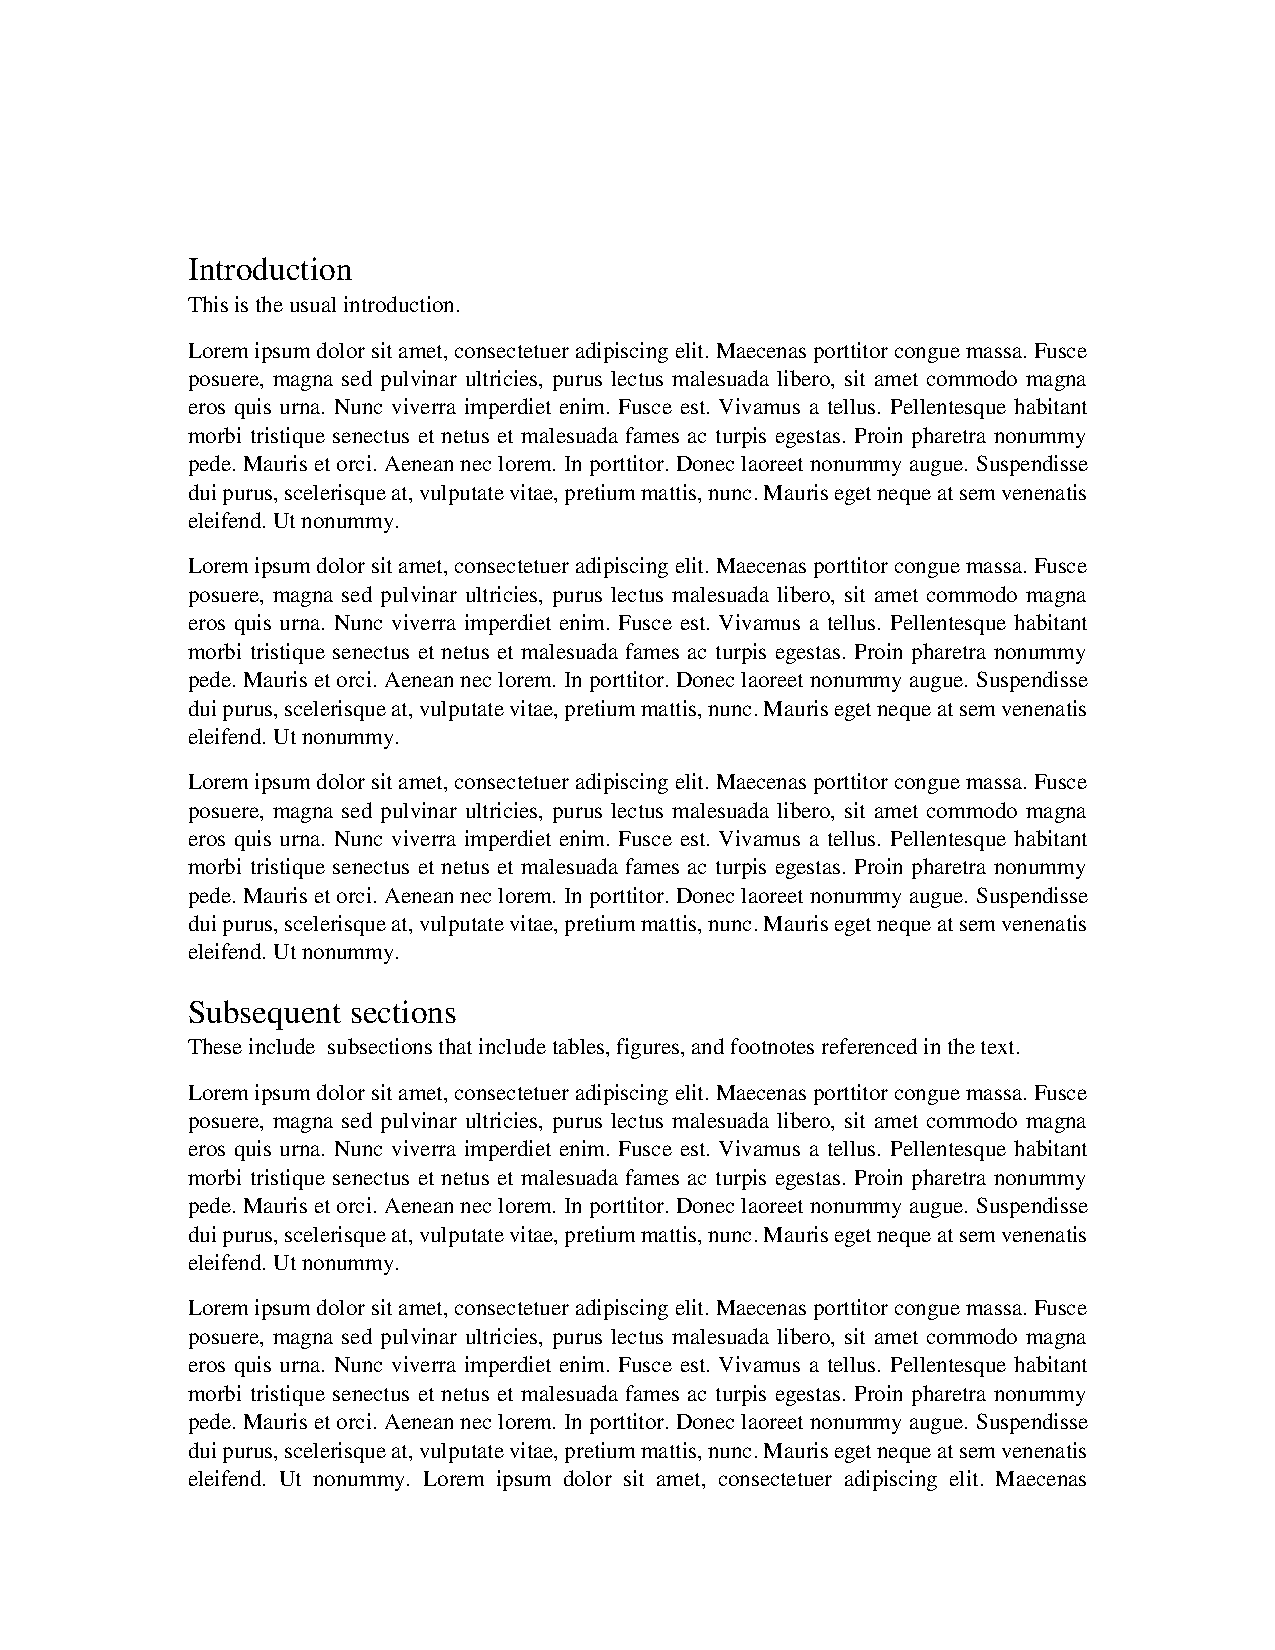
\includepdf[pages=-,offset=0 0.7in,pagecommand={}]{sample-word.pdf}
%\newpage
%Lorem ipsum
%\newpage
%Lorem ipsum
\end{document}
